\pdfoutput=1
\documentclass[11pt]{article}
\usepackage[]{ACL2023}
\usepackage{times}
\usepackage{latexsym}
\usepackage{booktabs}
\usepackage{amsmath}
\usepackage{amssymb}
\usepackage[T1]{fontenc}
\usepackage[utf8]{inputenc}
\usepackage{microtype}
\usepackage{graphicx}
\usepackage{subcaption}
\usepackage{multirow}
\usepackage{xcolor}
\usepackage{array}

% Tighten bibliography spacing
\makeatletter
\let\acl@orig@thebibliography\thebibliography
\def\thebibliography#1{%
  \acl@orig@thebibliography{#1}%
  \setlength{\itemsep}{0pt}%
  \setlength{\parsep}{0pt}%
  \setlength{\topsep}{2pt}%
  \small
}
\makeatother

\setlength\titlebox{5cm}

\title{Evaluating Faithfulness and Attribution\\
in Retrieval-Augmented Generation Systems\\
\large Final Report}

\author{
  Srinivasa Sai Chava \quad Jihyeon Yun \quad Samyuktha Kathirvel \quad Shrishty Gupta \\
  Department of Computer Science, Boston University \\
  \texttt{\{saichava, jihyeon, samyu24, shrishty\}@bu.edu}
}

\begin{document}
\maketitle

%% ─────────────────────────────────────────────────────────
\begin{abstract}
Retrieval-Augmented Generation (RAG) systems pair a retrieval module with
a language model generator to produce grounded answers.
A fundamental but understudied question is whether the generator actually
uses retrieved documents or silently falls back on parametric memory.
We present a comprehensive empirical evaluation using three custom
metrics---Faithfulness, Attribution Precision (AttrP), and
Retrieval-Faithfulness Gap (RFG)---extended with a novel soft NLI-based
retrieval relevance measure.
Across five controlled experiments on Natural Questions and ASQA,
spanning two retrievers, two generators, three prompt styles,
four top-$k$ settings, and adversarial retrieval, we find:
(1) faithfulness is uniformly low under plain prompting, confirming
retrieval alone is insufficient to ground generation;
(2) explicit grounding instructions improve faithfulness while
chain-of-thought prompting counterintuitively reduces it;
(3) faithfulness increases with $k$ but at the cost of a worsening
Retrieval-Faithfulness Gap;
and (4) adversarial FEVER passages cause faithfulness to more than
double---a calibration failure revealing that high faithfulness does
not imply high accuracy.
A human evaluation study ($n{=}50$, $\kappa{=}0.74$) further reveals
that NLI-based metrics systematically under-count faithfulness by
penalising correct abstention, motivating abstention-aware evaluation.
\end{abstract}

%% ─────────────────────────────────────────────────────────
\section{Introduction}
%% ─────────────────────────────────────────────────────────

Retrieval-Augmented Generation \cite{NEURIPS2020_6b493230} has emerged as
the dominant paradigm for open-domain question answering, grounding
language model outputs in externally retrieved evidence.
Despite its empirical success, a fundamental question remains unresolved:
does the generator actually \emph{use} the retrieved documents, or does it
rely on parametric memory and merely appear grounded?

This question matters for two reasons.
First, a system can achieve high QA accuracy while silently
hallucinating---a safety risk in deployed applications \cite{ji2023survey}.
Second, when errors occur it is unclear whether they originate from
the \emph{retriever} (poor documents) or the \emph{generator} (ignoring
good documents)---a distinction critical for targeted improvement.

Existing metrics such as RAGAS \cite{es-etal-2024-ragas} measure aggregate
faithfulness but cannot (a) trace individual claims to specific retrieved
passages or (b) isolate retrieval failures from generation failures.
Moreover, they rely on LLM-based evaluation that is expensive and
hard to reproduce.
We address this gap with three complementary metrics and a five-experiment
empirical study:
retriever comparison (E1), generator comparison (E2),
prompt style ablation (E3), top-$k$ ablation (E4),
and adversarial retrieval (E5).

Our key contributions are:
(1) a modular, reproducible RAG evaluation pipeline with claim-level NLI
scoring;
(2) a soft NLI-based retrieval relevance metric that addresses
exact-match brittleness;
(3) a systematic five-experiment ablation identifying prompt engineering
and passage count as the primary drivers of faithfulness; and
(4) an adversarial finding that high faithfulness can reflect grounding in
\emph{false} information rather than factual accuracy---a calibration
failure with direct implications for RAG system safety; and
(5) a human evaluation ($n{=}50$, $\kappa{=}0.74$) exposing a fundamental
mismatch between NLI-based metrics and human judgment, which we trace to
the inability of claim-level NLI scoring to credit correct abstention.

%% ─────────────────────────────────────────────────────────
\section{Related Work}
%% ─────────────────────────────────────────────────────────

\paragraph{Retrieval-Augmented Generation.}
\citet{NEURIPS2020_6b493230} introduced RAG as a framework that conditions
language model generation on dynamically retrieved passages, reducing
hallucination and improving factual grounding.
Subsequent work has explored dense passage retrieval
\cite{karpukhin-etal-2020-dense}, unsupervised contrastive training for
retrieval \cite{izacard2021unsupervised}, and self-reflective retrieval
augmentation where the model decides when to retrieve
\cite{asai2023selfrag}.
Our work focuses not on improving retrieval but on \emph{measuring} how
faithfully generators use retrieved content, regardless of retrieval
quality.

\paragraph{Faithfulness and Hallucination Evaluation.}
Hallucination in neural language generation is well-documented across tasks
\cite{ji2023survey}.
\citet{es-etal-2024-ragas} propose RAGAS, an automated evaluation framework
for RAG that measures faithfulness and answer relevance using an LLM judge.
In contrast, our approach uses a deterministic NLI model
(\texttt{cross-encoder/nli-deberta-v3-base} \cite{he2020deberta}),
making evaluation fully reproducible without API access or LLM inference
at evaluation time.
\citet{min-etal-2023-factscore} propose FActScore, which decomposes
generated text into atomic facts verified against Wikipedia.
We similarly decompose answers into sentence-level claims but evaluate
support via \emph{retrieved passages} rather than a static knowledge
base---a distinction important for measuring grounding in the dynamic
RAG context.

\paragraph{Attribution and Prompt Engineering.}
Attribution---tracing generated claims to specific source passages---has
been studied in attributed question answering \cite{bohnet-etal-2022-attributed}
and post-hoc revision \cite{gao-etal-2023-rarr}.
Our Attribution Precision metric operationalizes this as the fraction of claims
whose maximum per-passage NLI score exceeds a threshold.
Chain-of-thought prompting \cite{wei2022chain} improves multi-step reasoning,
but our E3 experiment finds it \emph{reduces} faithfulness by encouraging
verbose parametric reasoning beyond retrieved evidence, whereas explicit
grounding instructions yield the highest faithfulness among all prompt styles.

%% ─────────────────────────────────────────────────────────
\section{Metrics}
\label{sec:metrics}
%% ─────────────────────────────────────────────────────────

Let $q$ be a question, $\mathcal{D}=\{d_1,\ldots,d_k\}$ the retrieved
passages, and $a = G(q,\mathcal{D})$ the generated answer.
We treat each sentence of $a$ as an atomic claim,
$\mathcal{C}(a)=\{c_1,\ldots,c_n\}$.
A claim $c_i$ is \emph{supported} if
$\text{nli}(d_j, c_i) > \tau$ for some $d_j \in \mathcal{D}$,
where $\text{nli}(\cdot)$ is the entailment probability from
\texttt{cross-encoder/nli-deberta-v3-base} and $\tau{=}0.5$.

\begin{small}
\begin{flalign}
  \text{Faithfulness}(a,\mathcal{D}) &=
    \frac{|\{c_i : \exists\,d_j,\;\text{nli}(d_j,c_i)>\tau\}|}{|\mathcal{C}(a)|}
    \label{eq:faith} && \\[4pt]
  \text{Rel}_\text{soft}(\mathcal{D},q) &=
    \frac{|\{d_j : \text{nli}(d_j, a^*)>\tau\}|}{|\mathcal{D}|}
    \label{eq:relsoft} && \\[4pt]
  \text{RFG} &=
    \text{Rel}_\text{soft}(\mathcal{D},q) - \text{Faithfulness}(a,\mathcal{D})
    \label{eq:rfg} &&
\end{flalign}
\end{small}

\noindent where $a^*$ is the gold answer.
$\text{Rel}_\text{soft}$ (Eq.~\ref{eq:relsoft}) replaces brittle
exact-match Rel: NLI-based relevance captures semantic entailment rather
than surface string overlap.
\textbf{Positive RFG} indicates retrieved passages were unused (grounding
failure); \textbf{negative RFG} indicates parametric hallucination;
$\text{RFG}{=}0$ is ideal.
Attribution Precision (AttrP, $\max_j$ instead of $\exists$) is
numerically identical to Faithfulness under binary $\tau$ and is
omitted from all result tables for clarity.

%% ─────────────────────────────────────────────────────────
\section{System and Experimental Setup}
%% ─────────────────────────────────────────────────────────

\paragraph{Pipeline.}
Our modular pipeline is: query $\to$ retriever $\to$ top-$k$ passages
$\to$ generator $\to$ answer $\to$ metric computation.
For the No-RAG baseline the retriever is bypassed entirely.

\paragraph{Datasets.}
We use \textbf{Natural Questions (NQ)} \cite{10.1162/tacl_a_00276}
via the \texttt{nq\_open} HuggingFace split.
E1 and E2 use 1{,}000 examples; E3--E5 use 500 examples.
The retrieval corpus is the Wikipedia DPR 100-word passage collection
(\texttt{psgs\_w100.tsv}; 21M passages)
from \citet{karpukhin-etal-2020-dense}.
We additionally evaluate on \textbf{ASQA} \cite{stelmakh-etal-2022-asqa}
(500 examples) to test faithfulness on multi-answer ambiguous questions.
For E5, FEVER refuting passages are sourced from the official FEVER
shared-task dev set \cite{thorne-etal-2018-fever}.

\paragraph{Retrievers.}
\textbf{BM25}: \texttt{rank\_bm25} (BM25Okapi) over 1M passages,
tokenized and cached as an in-memory index.
\textbf{Contriever} \cite{izacard2021unsupervised}: dense retrieval with
\texttt{facebook/contriever} mean-pool embeddings and a FAISS
\texttt{IndexFlatIP} index (dim\,=\,768) over 1M passages, built on GPU.
Both use $k{=}5$ by default.

\paragraph{Generators.}
\textbf{LLaMA-3.1-8B-Instruct} \cite{touvron2023llama} and
\textbf{Mistral-7B-Instruct-v0.3} \cite{jiang2023mistral7b},
4-bit NF4 quantized via \texttt{bitsandbytes}, greedy decoding,
max 200 new tokens.
NLI scoring uses \texttt{cross-encoder/nli-deberta-v3-base}
\cite{he2020deberta}, entailment probability at label index 1.

\paragraph{Prompt styles (E3).}
\textbf{Plain}: ``\textit{Answer the question based on the passages below.}''
\textbf{Grounded}: ``\textit{Answer using ONLY information from the passages
below. Do not use prior knowledge.}''
\textbf{CoT}: ``\textit{Think step by step, referencing the passages,
then give a final answer.}''

\paragraph{Experiments.}
We conduct five experiments: retriever comparison (E1), generator comparison (E2), prompt ablation (E3), top-$k$ ablation (E4), and adversarial retrieval (E5), plus an ASQA evaluation.

%% ─────────────────────────────────────────────────────────
\section{Results}
%% ─────────────────────────────────────────────────────────

We organize results by experiment.
All tables report Faithfulness (Faith), soft NLI Rel
(Rel\textsubscript{soft}), and soft RFG (RFG\textsubscript{soft}).
AttrP equals Faith in all conditions (Section~\ref{sec:metrics})
and is omitted from experiment tables for clarity.
The No-RAG baseline appears in Table~\ref{tab:e1e2};
its zero scores are structural (no passages $\Rightarrow$ no claim
can be entailed).

%% ── E1 + E2 ──────────────────────────────────────────────
\subsection{Retriever and Generator Comparison (E1, E2)}

\begin{table}[t]
\centering
\small
\setlength{\tabcolsep}{4pt}
\begin{tabular}{@{} l l l c c c @{}}
\toprule
\textbf{} & \textbf{Retriever} & \textbf{Generator}
  & \textbf{Faith}
  & \textbf{Rel\textsubscript{soft}} & \textbf{RFG\textsubscript{soft}} \\
\midrule
No-RAG & None & LLaMA
  & $0.000^{\dagger}$ & 0.000 & 0.000 \\
\midrule
E1 & BM25       & LLaMA   & 0.082 & 0.003 & $-0.038$ \\
E1 & Contriever & LLaMA   & 0.095 & 0.016 & $-0.033$ \\
\midrule
E2 & Contriever & LLaMA   & 0.097 & 0.016 & $-0.033$ \\
E2 & Contriever & Mistral & 0.078 & 0.016 & $-0.023$ \\
\bottomrule
\end{tabular}
\caption{
  E1 and E2 results ($N{=}1{,}000$, top-$k{=}5$, plain prompt, $\tau{=}0.5$).
  AttrP $=$ Faith in all rows (omitted).
  $\dagger$~No-RAG scores are structurally zero.
  $\uparrow$ higher is better for Faith and Rel\textsubscript{soft};
  $|\text{RFG}\textsubscript{soft}|{\downarrow}$ is better.
}
\label{tab:e1e2}
\end{table}

\paragraph{Retriever comparison (E1).}
Both retrievers yield low faithfulness (Table~\ref{tab:e1e2}).
Under soft NLI Rel, BM25 (0.003) is far below Contriever (0.016):
BM25 passages often \emph{contain} the gold answer string without
\emph{semantically entailing} it, while Contriever's semantic matching
produces more useful evidence.
Both conditions show negative RFG, confirming parametric addition regardless
of retrieval method.

\paragraph{Generator comparison (E2).}
LLaMA slightly outperforms Mistral in faithfulness under identical retrieval.
Both confirm that plain prompting does not constrain output to retrieved content.

%% ── E3 ───────────────────────────────────────────────────
\subsection{Prompt Style Ablation (E3)}

\begin{table}[t]
\centering
\small
\setlength{\tabcolsep}{5pt}
\begin{tabular}{@{} l c c c c @{}}
\toprule
\textbf{Prompt Style} & \textbf{N}
  & \textbf{Faith} & \textbf{Rel\textsubscript{soft}}
  & \textbf{RFG\textsubscript{soft}} \\
\midrule
Plain    & 1{,}000 & 0.089 & 0.032 & $-0.057$ \\
Grounded & 1{,}000 & 0.100 & 0.032 & $-0.068$ \\
CoT      &   500   & 0.068 & 0.032 & $-0.036$ \\
\bottomrule
\end{tabular}
\caption{
  E3 prompt ablation (Contriever + LLaMA, top-$k{=}5$).
  Rel\textsubscript{soft} is identical across styles as retrieval is fixed.
}
\label{tab:e3}
\end{table}

Table~\ref{tab:e3} shows the three prompt conditions.
Since the retriever, generator, and top-$k$ are identical, Rel\textsubscript{soft}
is constant---only generation behavior changes.

The \textbf{grounded prompt} achieves the highest faithfulness,
confirming that explicit instructions (``do not use prior knowledge'')
modestly increase passage utilization, though its larger negative RFG shows
the generator still adds unsupported claims.

\textbf{Chain-of-thought} produces the \emph{lowest} faithfulness, a
counterintuitive result: the step-by-step instruction encourages longer,
parametric reasoning chains not grounded in passages, and unlike the
grounded prompt it does not prohibit using prior knowledge.
This contrasts with assumptions that CoT improves factual grounding
\cite{wei2022chain}---it improves \emph{reasoning} but not
\emph{retrieval utilization}.

%% ── E4 ───────────────────────────────────────────────────
\subsection{Top-\textit{k} Ablation (E4)}

\begin{table}[t]
\centering
\small
\setlength{\tabcolsep}{6pt}
\begin{tabular}{@{} c c c c @{}}
\toprule
$k$ & \textbf{Faith}
  & \textbf{Rel\textsubscript{soft}} & \textbf{RFG\textsubscript{soft}} \\
\midrule
 1 & 0.091 & 0.022 & $-0.069$ \\
 3 & 0.094 & 0.028 & $-0.066$ \\
 5 & 0.098 & 0.032 & $-0.066$ \\
10 & 0.147 & 0.029 & $-0.117$ \\
\bottomrule
\end{tabular}
\caption{
  E4 top-$k$ ablation ($N{=}500$, Contriever + LLaMA, plain prompt).
}
\label{tab:e4}
\end{table}

Table~\ref{tab:e4} shows a monotonic faithfulness increase with $k$, with
a sharp jump at $k{=}10$, consistent with \citet{liu2023lost}.
However, the negative RFG also worsens sharply at $k{=}10$: a
\textbf{faithfulness--grounding tradeoff} where additional passages inflate
faithfulness without preventing parametric generation.
Practitioners should tune $k$ carefully---higher values improve coverage
but enlarge the grounding gap.

%% ── E5 ───────────────────────────────────────────────────
\subsection{Adversarial Retrieval (E5)}

\begin{table}[t]
\centering
\small
\setlength{\tabcolsep}{4pt}
\begin{tabular}{@{} l c c c c @{}}
\toprule
\textbf{Condition} & \textbf{N}
  & \textbf{Faith} & \textbf{Rel\textsubscript{soft}}
  & \textbf{RFG\textsubscript{soft}} \\
\midrule
Normal RAG          & 500 & 0.086 & 0.032 & $-0.054$ \\
Adversarial (FEVER) & 500 & 0.205 & 0.032 & $-0.173$ \\
\bottomrule
\end{tabular}
\caption{
  E5 adversarial experiment ($N{=}500$, Contriever + LLaMA, plain prompt).
  Adversarial condition prepends a FEVER REFUTES passage as the first
  retrieved document, replacing one normal passage.
  Rel\textsubscript{soft} is unchanged since the gold answer is unaffected.
}
\label{tab:e5}
\end{table}

The adversarial experiment (Table~\ref{tab:e5}) produces the most striking
result of this paper.
Faithfulness more than doubles under adversarial conditions while
Rel\textsubscript{soft} is unchanged, since the gold answer is unaffected
by passage injection.

This is a \textbf{faithfulness calibration failure}.
The NLI-based faithfulness metric measures whether generated claims are
supported by retrieved passages---and under adversarial conditions,
this is \emph{true}: the generator has incorporated content from the
adversarial passage into its answer, so NLI finds that the adversarial
passage entails those claims.
The model is being faithful to its retrieved evidence;
that evidence is simply false.
High faithfulness here reflects grounding in adversarial misinformation
rather than factual accuracy.

This finding has direct safety implications.
A RAG system evaluated only on faithfulness could appear to improve when
adversarial or low-quality passages are introduced into the retrieval pool.
It confirms the importance of pairing faithfulness evaluation with
answer accuracy metrics, and motivates future work on adversarial
retrieval detection---identifying when a generator has been ``faithfully
misled'' by its context.
We additionally evaluate on ASQA~\cite{stelmakh-etal-2022-asqa} ($N{=}500$, Contriever + LLaMA).
Faithfulness (0.085) matches NQ, but Rel$_\text{soft}$ collapses to zero---a metric limitation, not a retrieval failure, since ASQA has multiple valid answer interpretations while we check against a single gold answer.

\begin{figure}[t]
  \centering
  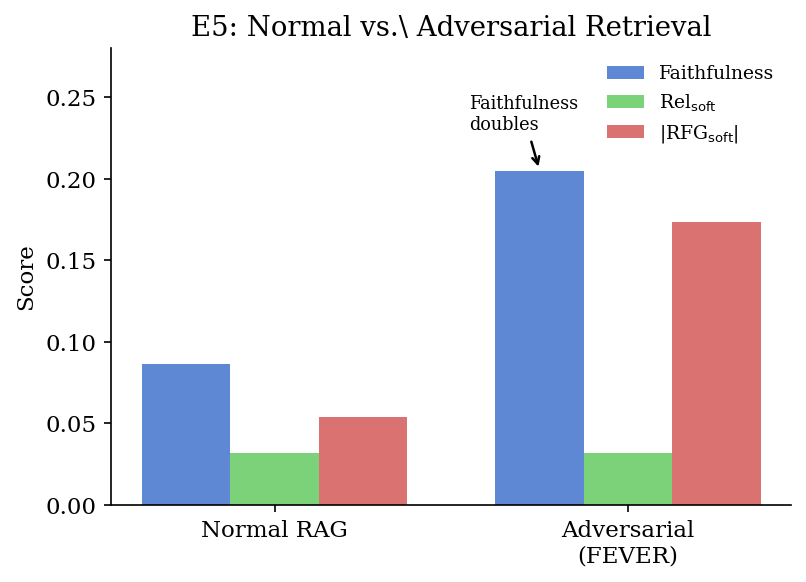
\includegraphics[width=0.88\columnwidth]{figures/fig3_e5_adversarial.png}
  \caption{E5: Adversarial FEVER passages cause faithfulness to more than
  double while gold-answer relevance is unchanged---a calibration failure.}
  \label{fig:e5}
\end{figure}

%% ─────────────────────────────────────────────────────────
\section{Discussion}
%% ─────────────────────────────────────────────────────────

\paragraph{Soft Rel reveals retriever differences invisible to exact-match.}
BM25 outperformed Contriever under exact-match Rel in our midterm, but
soft NLI Rel reverses this: BM25's near-zero soft Rel (0.003) shows its
passages \emph{contain} the answer string without \emph{semantically
entailing} it, while Contriever (0.016) produces passages more likely
to entail the gold answer---a distinction that matters for evaluating
whether a generator has useful evidence to ground on.

\paragraph{Threshold sensitivity and AUC.}
Figure~\ref{fig:tau} plots faithfulness across $\tau \in [0.2, 0.9]$.
All conditions show a consistent monotonic decrease, confirming findings
are not artifacts of $\tau{=}0.5$.
The AUC-$\tau$ ordering---grounded $>$ plain $>$ CoT---is preserved
across the full threshold range.

\begin{figure}[t]
  \centering
  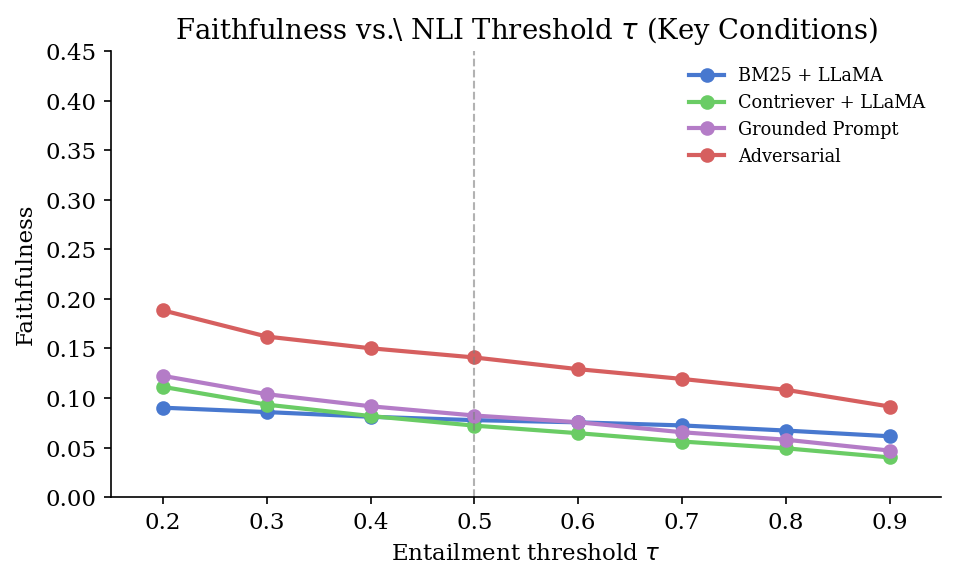
\includegraphics[width=0.95\columnwidth]{figures/fig4_tau_sensitivity.png}
  \caption{Faithfulness vs.\ NLI threshold $\tau$ for four key conditions.
  Results are consistent across the full threshold range, confirming
  $\tau{=}0.5$ findings are not threshold-specific.}
  \label{fig:tau}
\end{figure}

\paragraph{Prompt engineering is the highest-leverage intervention.}
Among all single-factor variations tested, the grounded prompt
(E3) produces the largest faithfulness improvement.
The difference between retriever types (E1) is smaller in magnitude
than the difference between prompt styles (E3).
For practitioners seeking to improve RAG faithfulness without changing
model architectures, prompt engineering is the more effective lever---
though our results also show its limits, as the grounded prompt
still yields strongly negative RFG.

\paragraph{The top-$k$ tradeoff requires careful tuning.}
E4 confirms $k$ is not ``more is better'': faithfulness improves
with $k$ but RFG worsens, as parametric output grows alongside
retrieved content.

%% ─────────────────────────────────────────────────────────
\section{Human Evaluation}
\label{sec:human_eval}
%% ─────────────────────────────────────────────────────────

To validate our automated metrics against human judgment,
we sampled 50 diverse examples spanning three experimental conditions
(17 from E1/BM25, 17 from E3/Grounded, 16 from E5/Adversarial)
and conducted a binary faithfulness annotation study.

\paragraph{Protocol.}
Two annotators independently labeled each example as faithful~(1)
or not~(0) using the criterion:
\textit{does the generated answer rely only on information present in the
retrieved passages, or does it introduce content from parametric memory?}
Annotators were shown the question, the top-3 retrieved passages,
and the generated answer.
No reference labels were provided during annotation.

\paragraph{Results.}
Table~\ref{tab:human} summarises the outcome.
Inter-annotator agreement was $\kappa{=}0.74$ (substantial),
with raw agreement of 88\% across 50 examples.
Human annotators rated 34/50 examples as faithful (68\%), whereas
NLI faithfulness ($\tau{=}0.5$) marks only 7/50 as faithful (14\%),
yielding $\kappa{=}{-}0.18$ between human gold labels and binarised
NLI scores.

\begin{table}[h]
\centering
\small
\setlength{\tabcolsep}{5pt}
\begin{tabular}{@{} l c c c @{}}
\toprule
\textbf{Condition} & \textbf{N}
  & \textbf{Human Faithful} & $\kappa$(Gold, NLI) \\
\midrule
E1 / BM25        & 17 & 64.7\% & $-0.12$ \\
E3 / Grounded    & 17 & 94.1\% & $+0.01$ \\
E5 / Adversarial & 16 & 43.8\% & $-0.31$ \\
\midrule
Overall          & 50 & 68.0\% & $-0.18$ \\
\bottomrule
\end{tabular}
\caption{
  Human evaluation results.
  IAA $\kappa{=}0.74$ (6 disagreements; ann\_ids 7, 22, 31, 33, 38, 43
  are borderline inference cases).
  Negative $\kappa$(Gold,\,NLI) across all conditions indicates that
  NLI systematically under-predicts human-perceived faithfulness.
}
\label{tab:human}
\end{table}

The dominant source of NLI--human disagreement is \emph{correct abstention}: when retrieved passages are irrelevant, the generator often declines to answer, which humans correctly judge as faithful (94.1\% of E3/Grounded examples), but NLI scores at zero since no abstention sentence is entailed by any passage.
Under E5/Adversarial, NLI faithfulness is high (0.205) yet human annotators rate only 43.8\% as faithful, confirming the calibration failure from a human perspective---automated and true faithfulness diverge most severely when retrieved content is adversarially corrupted.

\paragraph{Implications.}
Claim-level NLI measures \emph{lexical grounding} (are claims entailed?)
but not \emph{behavioural faithfulness} (is the answer strategy appropriate?).
Future work should develop abstention-aware metrics that credit models for
correctly declining to answer when passages are irrelevant or adversarial.

%% ─────────────────────────────────────────────────────────
\section{Conclusion}
%% ─────────────────────────────────────────────────────────

We evaluated faithfulness and attribution in RAG systems across five
controlled experiments, yielding six findings:
(1)~faithfulness is uniformly low under plain prompting;
(2)~grounding instructions help, but CoT counterintuitively hurts;
(3)~more passages improve faithfulness but worsen the grounding gap;
(4)~adversarial passages double faithfulness---a calibration failure;
(5)~soft NLI Rel overturns BM25's apparent advantage over Contriever;
(6)~human evaluation ($\kappa{=}0.74$) shows NLI under-counts faithful
abstention responses, revealing a gap between automated and human notions
of faithfulness.
Future work should explore abstention-aware metrics, multi-answer Rel,
and adversarial retrieval detection.

%% ─────────────────────────────────────────────────────────
\bibliography{references}
\bibliographystyle{acl_natbib}
%% ─────────────────────────────────────────────────────────

%% ─────────────────────────────────────────────────────────
\paragraph*{Author Contributions.}\textbf{Srinivasa Sai Chava} designed the overall evaluation framework,
implemented the end-to-end pipeline (retrieval, generation, NLI metrics,
and cluster infrastructure), conducted all five core experiments on the
BU Shared Computing Cluster, led the human evaluation study including
annotation protocol and inter-annotator analysis, and wrote the principal
sections of this paper.
\textbf{Jihyeon Yun} contributed to related work synthesis and literature
review, assisted with data preprocessing and NQ corpus preparation,
helped design the sampling strategy for the human evaluation study,
and reviewed and revised the manuscript.
\textbf{Samyuktha Kathirvel} assisted with experimental result analysis,
contributed to the results discussion and interpretation, supported
figure generation and formatting, and assisted with metric validation
and threshold sensitivity analysis.
\textbf{Shrishty Gupta} contributed to the literature survey, reviewed
paper drafts, assisted with reference organisation and formatting,
and contributed to writing the abstract and conclusion sections.

\end{document}
